\documentclass[11pt]{beamer}  %% versione proiettore
%%\documentclass[11pt,handout]{beamer} %% versione stampa
\usepackage{Reflection}

\mode<article>
{
  \usepackage{fullpage}
  \usepackage{hyperref}
}

\mode<presentation>
{
  \setbeamertemplate{background canvas}[vertical shading][bottom=red!10,top=blue!10]
  \usetheme{Jb-2ed}
  \usefonttheme[onlysmall]{structurebold}
}

\title{Short Notes on Compiler Construction}
\author{Fausto Spoto, Universit\`a di Verona, Italy}
\date{July 2014}

\setbeamercovered{invisible}

\begin{document}

\frame{\titlepage}

\begin{frame}
\frametitle{Compilation into native code}

\begin{center}
\includegraphics[scale=0.6]{pictures/c_compiler.jpg}
\end{center}

\end{frame}

\begin{frame}
\frametitle{Compilation through an intermediate bytecode}

\begin{center}
\includegraphics[scale=0.6]{pictures/java_compiler.jpg}
\end{center}

\end{frame}

\begin{frame}
\frametitle{Compilation phases}

\begin{center}
\includegraphics[scale=0.4]{pictures/compilation_phases.jpg}
\end{center}

\end{frame}

\begin{frame}
\frametitle{Lexical analysis}

\begin{center}
My open source Kitten compiler: \texttt{https://github.com/HotMoka/Kitten}
\end{center}

\begin{center}
\begin{redbox}{Lexical analysis}
\begin{itemize}
\item \textbf{input:} textual source code
\item \textbf{output:} sequence of tokens
\item \textbf{error:} unknown token
\end{itemize}
\end{redbox}
\end{center}

\end{frame}

\begin{frame}[fragile]
\frametitle{Input: Kitten source code}

\vspace*{-2ex}
\begin{verbatim}
class Led {
  field boolean state
 
  constructor() {}

  method void on()
    this.state := true

  method void off()
    this.state := false

  method boolean isOn()
    return this.state

  method boolean isOff()
    return !this.state
}
\end{verbatim}

\end{frame}

\begin{frame}[fragile]
\frametitle{Output: sequence of tokens}

\begin{verbatim}
CLASS from 0 to 4
ID(Led) from 6 to 8
LBRACE from 10 to 10
FIELD from 14 to 18
BOOLEAN from 20 to 26
ID(state) from 28 to 32
CONSTRUCTOR from 37 to 47
LPAREN from 48 to 48
RPAREN from 49 to 49
LBRACE from 51 to 51
RBRACE from 52 to 52
METHOD from 57 to 62
VOID from 64 to 67
ID(on) from 69 to 70
...
\end{verbatim}

\end{frame}

\begin{frame}\frametitle{Old friends: Regular expressions}

\begin{greenbox}{}
An \emph{alphabet} $\Lambda$ is a finite collection of symbols (\emph{characters})
\end{greenbox}

\mbox{}\\

\begin{greenbox}{Regular Expressions $\mathcal{R}$ over $\Lambda$}
\begin{itemize}
\item $\emptyset\in\mathcal{R}$ (empty set)
\item $\varepsilon\in\mathcal{R}$ (empty string)
\item $\Lambda\subseteq\mathcal{R}$ (single characters)
\item if $r_1,r_2\in\mathcal{R}$ then $r_1r_2\in\mathcal{R}$ (sequence)
\item if $r_1,r_2\in\mathcal{R}$ then $r_1|r_2\in\mathcal{R}$ (union)
\item if $r\in\mathcal{R}$ then $r^*\in\mathcal{R}$ (iteration)
\end{itemize}

\end{greenbox}

\end{frame}

\begin{frame}\frametitle{A regular expression denotes a language}

\begin{greenbox}{}
\begin{itemize}
\item $\mathcal{L}(\emptyset)=\emptyset$
\item $\mathcal{L}(\varepsilon)=\{\varepsilon\}$
\item $\mathcal{L}(a)=\{a\}$ for every $a\in\Lambda$
\item $\mathcal{L}(r_1r_2)=\{s_1s_2\mid s_1\in\mathcal{L}(r_1)\text{ and }
      s_2\in\mathcal{L}(r_2)\}$
\item $\mathcal{L}(r_1|r_2)=\mathcal{L}(r_1)\cup\mathcal{L}(r_2)$
\item $\mathcal{L}(r^*)=\{s_1\cdots s_n\mid n\ge 0\text{ and }s_i\in
      \mathcal{L}(r)\text{ for all }0\le i\le n\}$.
\end{itemize}
\end{greenbox}

\mbox{}\\

\begin{pinkbox}{For instance}
\begin{itemize}
\item \texttt{then} denotes the keyword $\{\mathtt{then}\}$
\item \texttt{[a-zA-Z][a-zA-Z0-9\_]∗} denotes the identifiers
\end{itemize}
\end{pinkbox}

\end{frame}

\begin{frame}\frametitle{What you can \underline{not} do with regular expressions}

\begin{greenbox}{}
\begin{itemize}
\item you cannot define recursive languages
\item you cannot count (match parentheses)
\end{itemize}
\end{greenbox}

\begin{center}
C, Java, Kitten source code is defined in a recursive way and is correct only if
parentheses match
\end{center}

\end{frame}

\begin{frame}[fragile]\frametitle{Building a lexical analyzer with JLex}

$\mathtt{https://www.cs.princeton.edu/\ \tilde{}\ appel/modern/java/JLex/}$

\begin{center}
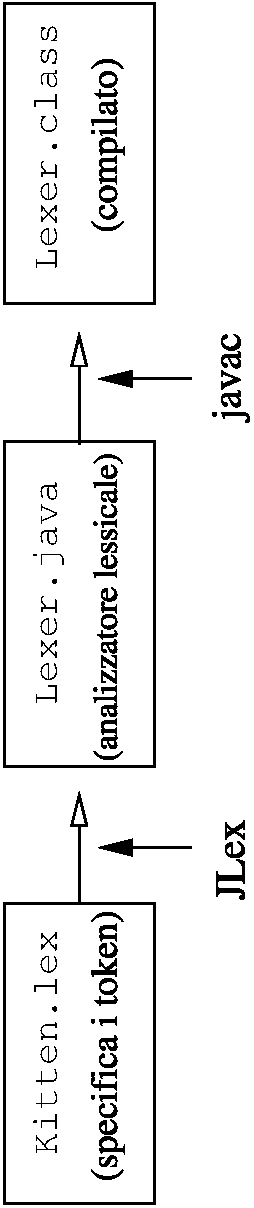
\includegraphics[scale=0.4]{pictures/jlex.pdf}
\end{center}

\begin{verbatim}
then                   {return tok(THEN, null);}
+                      {return tok(PLUS, null);}
:=                     {return tok(ASSIGN, null);}
[a-zA-Z][a-zA-Z0-9_]*  {return tok(ID, yytext());}
[0-9]+                 {return tok(INTEGER,
                              new Integer(yytext()));}
[0-9]*.[0-9]+          {return tok(FLOATING,
                              new Float(yytext()));}
\end{verbatim}

\end{frame}

\begin{frame}
\frametitle{Inside JLex}

\begin{enumerate}
\item regular expressions $\Rightarrow$ NFA
\item NFA $\Rightarrow$ DFA
\item DFA $\Rightarrow$ \texttt{Lexer.java}
\end{enumerate}

\mbox{}\\

\begin{greenbox}{Disambiguation rules}
\begin{itemize}
\item longest match
\item rule priority
\end{itemize}
\end{greenbox}

\end{frame}

\begin{frame}
\frametitle{Syntactical analysis}

\begin{center}
\begin{redbox}{Syntactical analysis}
\begin{itemize}
\item \textbf{input:} sequence of tokens
\item \textbf{output:} abstract syntax tree
\item \textbf{error:} syntax error
\end{itemize}
\end{redbox}
\end{center}

\end{frame}

\begin{frame}[fragile]
\frametitle{Input: sequence of tokens (yes, you have seen this already)}

\begin{verbatim}
CLASS from 0 to 4
ID(Led) from 6 to 8
LBRACE from 10 to 10
FIELD from 14 to 18
BOOLEAN from 20 to 26
ID(state) from 28 to 32
CONSTRUCTOR from 37 to 47
LPAREN from 48 to 48
RPAREN from 49 to 49
LBRACE from 51 to 51
RBRACE from 52 to 52
METHOD from 57 to 62
VOID from 64 to 67
ID(on) from 69 to 70
...
\end{verbatim}

\end{frame}

\begin{frame}\frametitle{Abstract syntax \emph{tree}}

\begin{center}
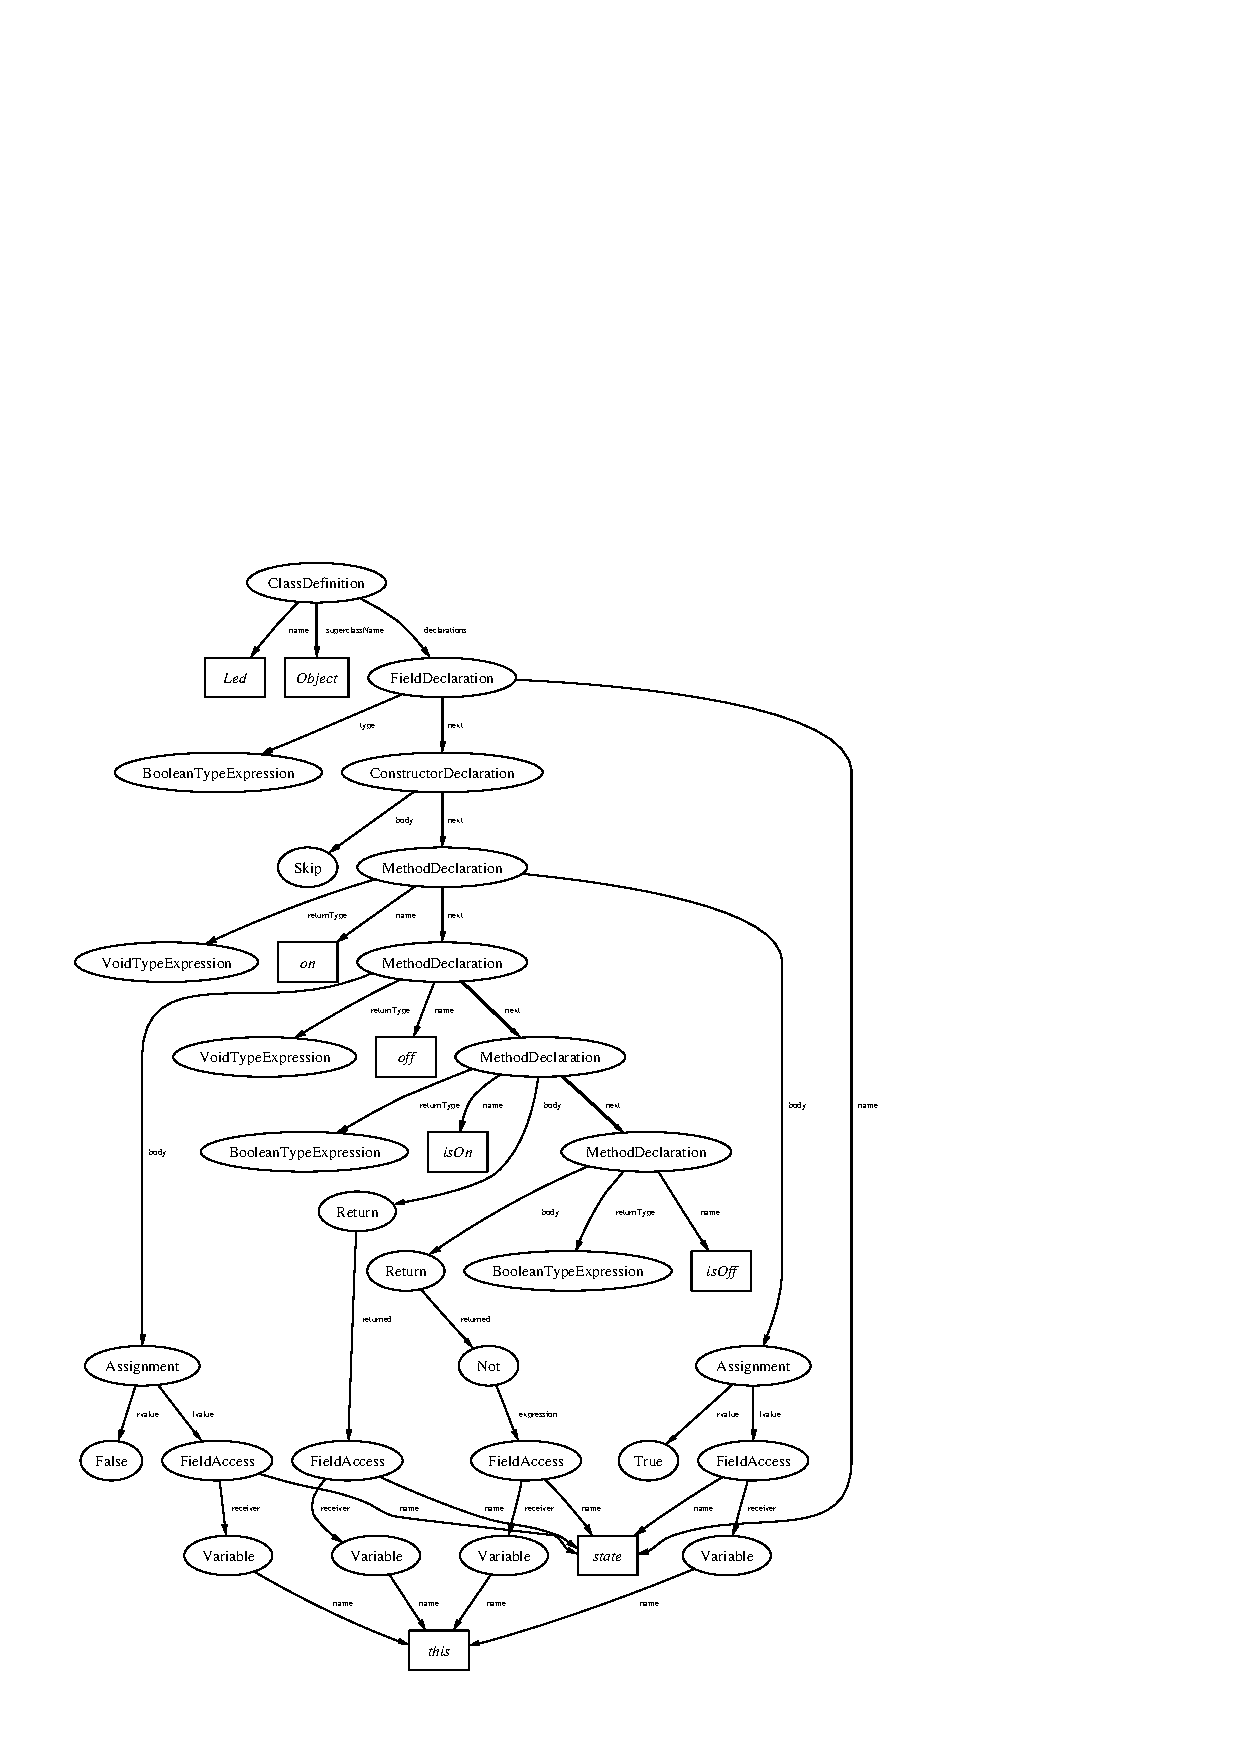
\includegraphics[scale=0.4]{pictures/led_logica.pdf}
\end{center}

\end{frame}

\begin{frame}\frametitle{A closer look 1/2}

\begin{center}
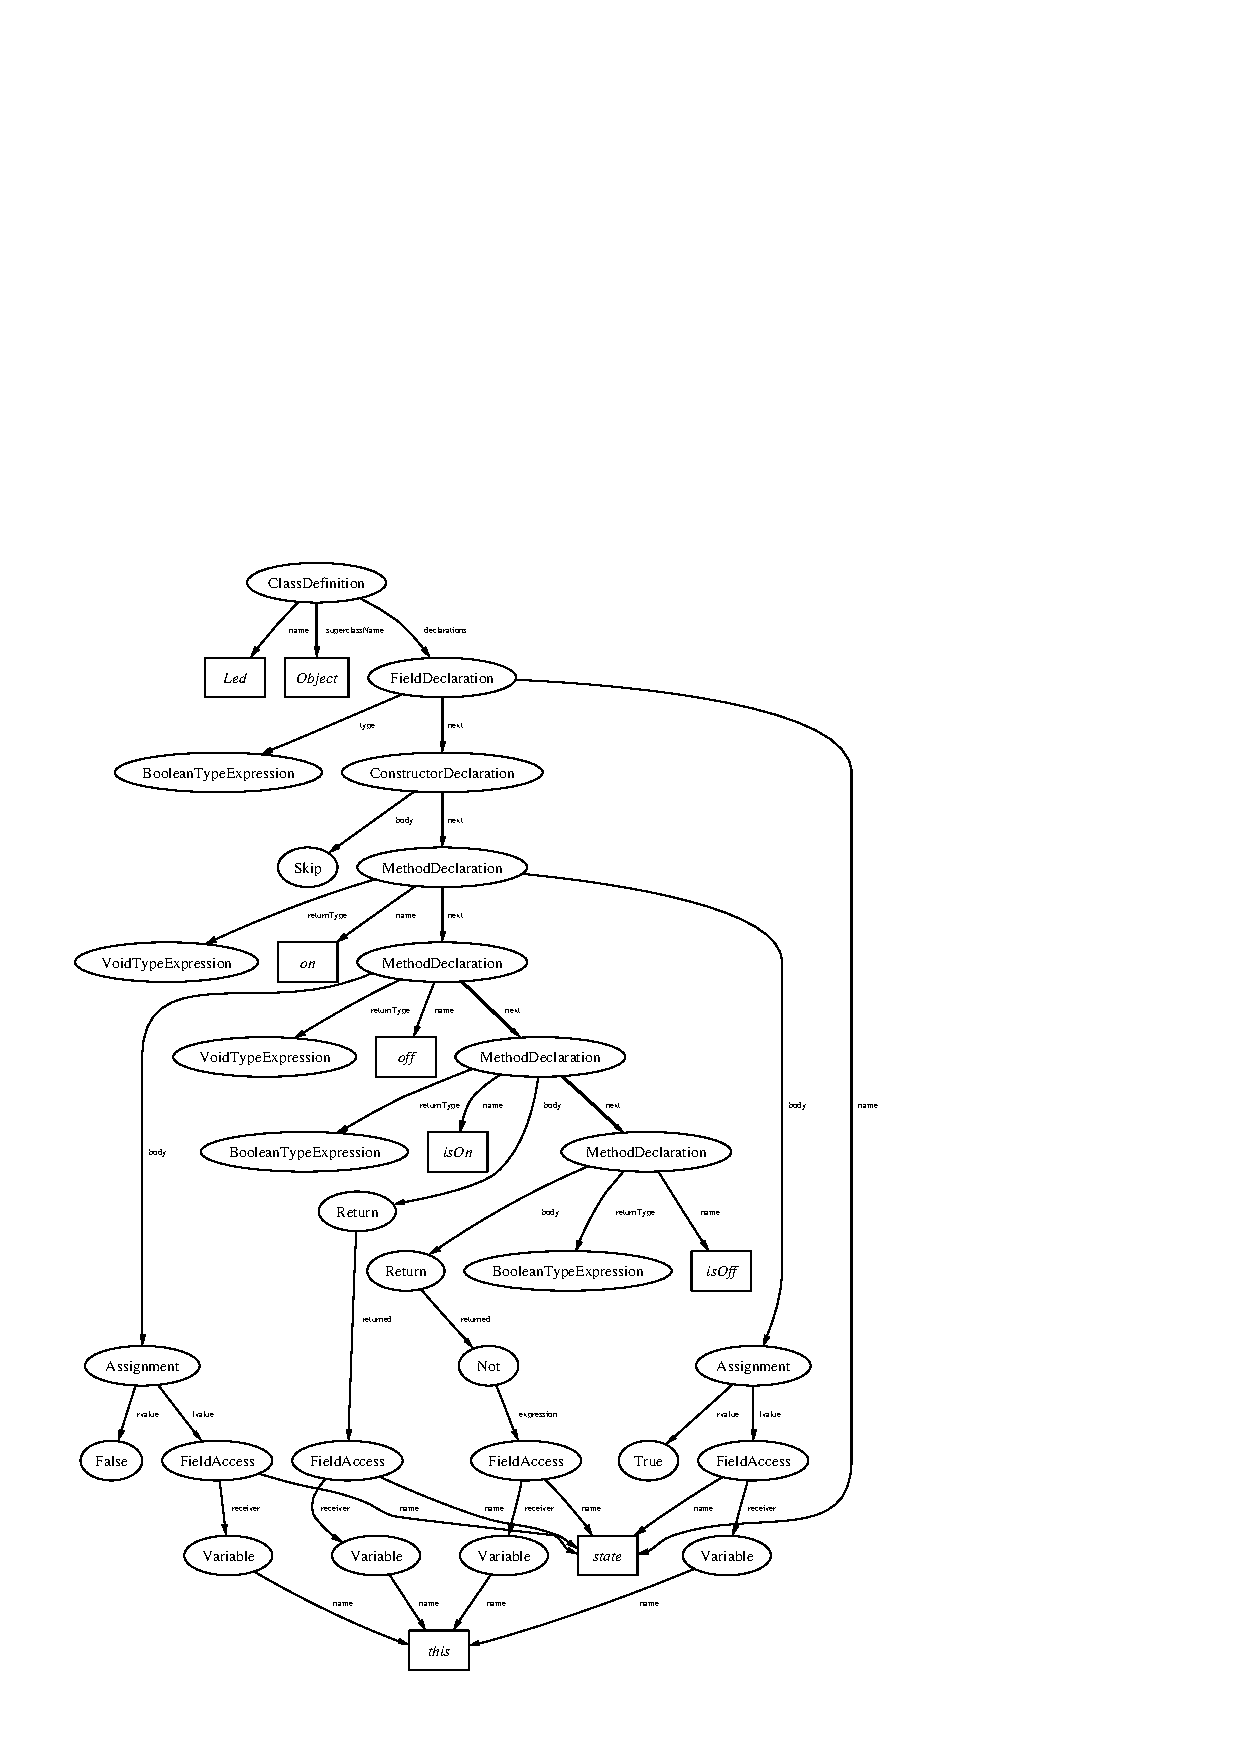
\includegraphics[scale=1]{pictures/led_logica.pdf}
\end{center}

\end{frame}

\begin{frame}\frametitle{A closer look 2/2}

\begin{center}
\includegraphics[scale=1]{pictures/led_logica_2.pdf}
\end{center}

\end{frame}

\begin{frame}\frametitle{Context-free grammars}

\begin{greenbox}{}
A \emph{context-free grammar} over an alphabet $\Lambda$
is a quadruple $\langle T,N,I,P\rangle$ where
\begin{itemize}
\item $T\subseteq\Lambda$
      is a set of \emph{terminals}
\item $N$ is a set of \emph{non-terminals}
\item $I\in N$ is the \emph{starting non-terminal}
\item $P$ is a set of \emph{productions}, that is, arrows such as
      $L\to\gamma$ where $L\in N$ and $\gamma\in (T\cup N)^*$.
\end{itemize}
\end{greenbox}

\mbox{}\\

For instance:
%
\[
\begin{split}
  T &= \{\mathtt{a},\mathtt{b}\}\\
  N &= \{I\}\\
  P &= \{I\to\varepsilon,\ I\to\mathtt{a}I\mathtt{b}\}
\end{split}
\]

\end{frame}

\begin{frame}\frametitle{Derivations}

\begin{greenbox}{}
Given $G=\langle T,N,I,P\rangle$ we say that
$\beta$ is
\emph{derived in $G$ in a step}
from $\alpha$ iff there is
$L\to\gamma\in P$ such that $\alpha=\eta L\delta$ and $\beta=\eta\gamma\delta$.
We write it as $\alpha\Rightarrow\beta$.
A \emph{derivation} for $G$ is a sequence of steps
$\alpha\Rightarrow\beta_1\Rightarrow\beta_2\ldots$.
\end{greenbox}

\mbox{}\\

For instance:
%
\begin{align*}
  \mathtt{ab}I\mathtt{b}&\Rightarrow\mathtt{aba}I\mathtt{bb}\\
  \mathtt{aba}I\mathtt{bb}&\Rightarrow\mathtt{ababb}\\
  I&\Rightarrow\mathtt{a}I\mathtt{b}\\
  I&\Rightarrow^*I\\
  \mathtt{ab}I\mathtt{b}&\Rightarrow^*\mathtt{ababb}.
\end{align*}

\end{frame}

\begin{frame}\frametitle{Language of a grammar}

\begin{greenbox}{}
Given a grammar $G$ on an alphabet $\Lambda$,
its language $L(G)$ is
\[
  L(G)=\{\alpha\text{ ground}\mid I\Rightarrow^*\alpha\}.
\]
\end{greenbox}

\mbox{}\\

For instance, for the previous example of grammar:
%
\[
  L(G)=\{\mathtt{a}^n\mathtt{b}^n\mid n\ge 0\}.
\]

\end{frame}

\begin{frame}\frametitle{Parse trees}

\begin{greenbox}{}
A \emph{parse tree} for $G=\langle T,N,I,P\rangle$ is a tree such that
%
\begin{enumerate}
\item its nodes are labeled with an element from $N$ or from $T$ or with
      $\varepsilon$;
\item its root is labeled with $I$
\item its leaves are labeled with elements from $T$ or with $\varepsilon$
\item for every node labeled with $L$ and its children labeled with
      $e_1,\ldots,e_n$ (left-to-right) we have $L\to e_1\cdots e_n\in P$.
\end{enumerate}
%
The frontier of the tree is the string derived by the tree from its root.
\end{greenbox}

\begin{center}
A parse tree stands for more derivations, by abstracting away the order or replacement of
the non-terminals
\end{center}

\end{frame}

\begin{frame}\frametitle{Ambiguity 1/2}

Consider the grammar
%
\[
\begin{split}
  I&\to\varepsilon\\
  I&\to\mathtt{a}\\
  I&\to\mathtt{b}\\
  I&\to II
\end{split}
\]
%
It admits two parse trees for the same word $\mathtt{abb}$:
%
\[
\xymatrix{
   &   & I\ar[ld]\ar[rd] \\
   & I\ar[ld]\ar[rd] &   & I\ar[d]\\
 I\ar[d] &   & I\ar[d] & \mathtt{b}\\
 \mathtt{a} & & \mathtt{b}
}
\qquad\qquad\qquad
\xymatrix{
  & I\ar[ld]\ar[rd] \\
I\ar[d] &   & I\ar[ld]\ar[rd]\\
\mathtt{a} & I\ar[d] &  & I\ar[d]\\
  & \mathtt{b} &  & \mathtt{b}
}
\]

\end{frame}

\begin{frame}\frametitle{Ambiguity 2/2}

\begin{pinkbox}{Why ambiguity is bad}
\begin{itemize}
\item Ambiguity means that the same word can be given two structures, that is, potentially,
      two distinct interpretations
\item With an ambiguous grammar, a compiler does not know which is the right interpretation of a program
\item In a perfect world, grammars should be non-ambiguous but this often entails that they become
      complex and innatural
\item We will give a concrete example later
\end{itemize}
\end{pinkbox}

\end{frame}

\begin{frame}[fragile]\frametitle{Recursive descent parsing}
%
\begin{align*}
  \mathit{I}&\to\mathit{com}\ \mathtt{\$} & \mathit{exp}&\to\mathtt{INTEGER}\\
  \mathit{com}&\to\mathit{exp}\ \mathtt{ASSIGN}\ \mathtt{INTEGER} & \mathit{exp}&\to\mathtt{ID}\\
  && \mathit{exp}&\to\mathtt{MINUS}\ \mathit{exp}
\end{align*}
%
We can implement it with a recursive descent parser:
%
\begin{verbatim}
public void parse() { parseI(); }
private void parseI() { parseCom(); eat(EOF); }
private void parseCom() { parseExp(); eat(ASSIGN); eat(INTEGER); }
private void parseExp() {
  switch (lookahead) {
    case ID: eat(ID); break;
    case INTEGER: eat(INTEGER); break;
    case MINUS: eat(MINUS); parseExp();
    default: syntax_error(lookahead);
  }
}
\end{verbatim}
\end{frame}

\begin{frame}\frametitle{When does recursive descent parsing fail?}

Recursive descent parsing fails
%
\begin{itemize}
\item when the first token is not enough to distinguish two productions for the same non-terminal
\item when the grammar is left-recursive
\end{itemize}

\mbox{}\\

For instance it fails for:
%
\begin{align*}
I&\to A\mathtt{\$}\\
A&\to\mathtt{a}\\
A&\to A\mathtt{a}
\end{align*}

In practice, it fails for the grammars of all sensible programming languages

\end{frame}

\begin{frame}\frametitle{$LR$ parsing}

\begin{greenbox}{}
$LR$ parsing uses a stack automaton to remember what has already been seen during parsing
and which are the possible productions that we can use in the future, depending on the
input token that will get processed by the compiler:

\begin{itemize}
\item details are long and boring: see any compilers book
\item the construction of the parser is automatic from the grammar
\item a special case of $LR$ parsing is the standard approach for compiler construction
\item it will anyway fail for ambiguous grammars
\end{itemize}

\end{greenbox}

\end{frame}

\begin{frame}\frametitle{Automatic parser generation with JavaCup}

$\mathtt{http://www2.cs.tum.edu/projects/cup/}$

\begin{center}
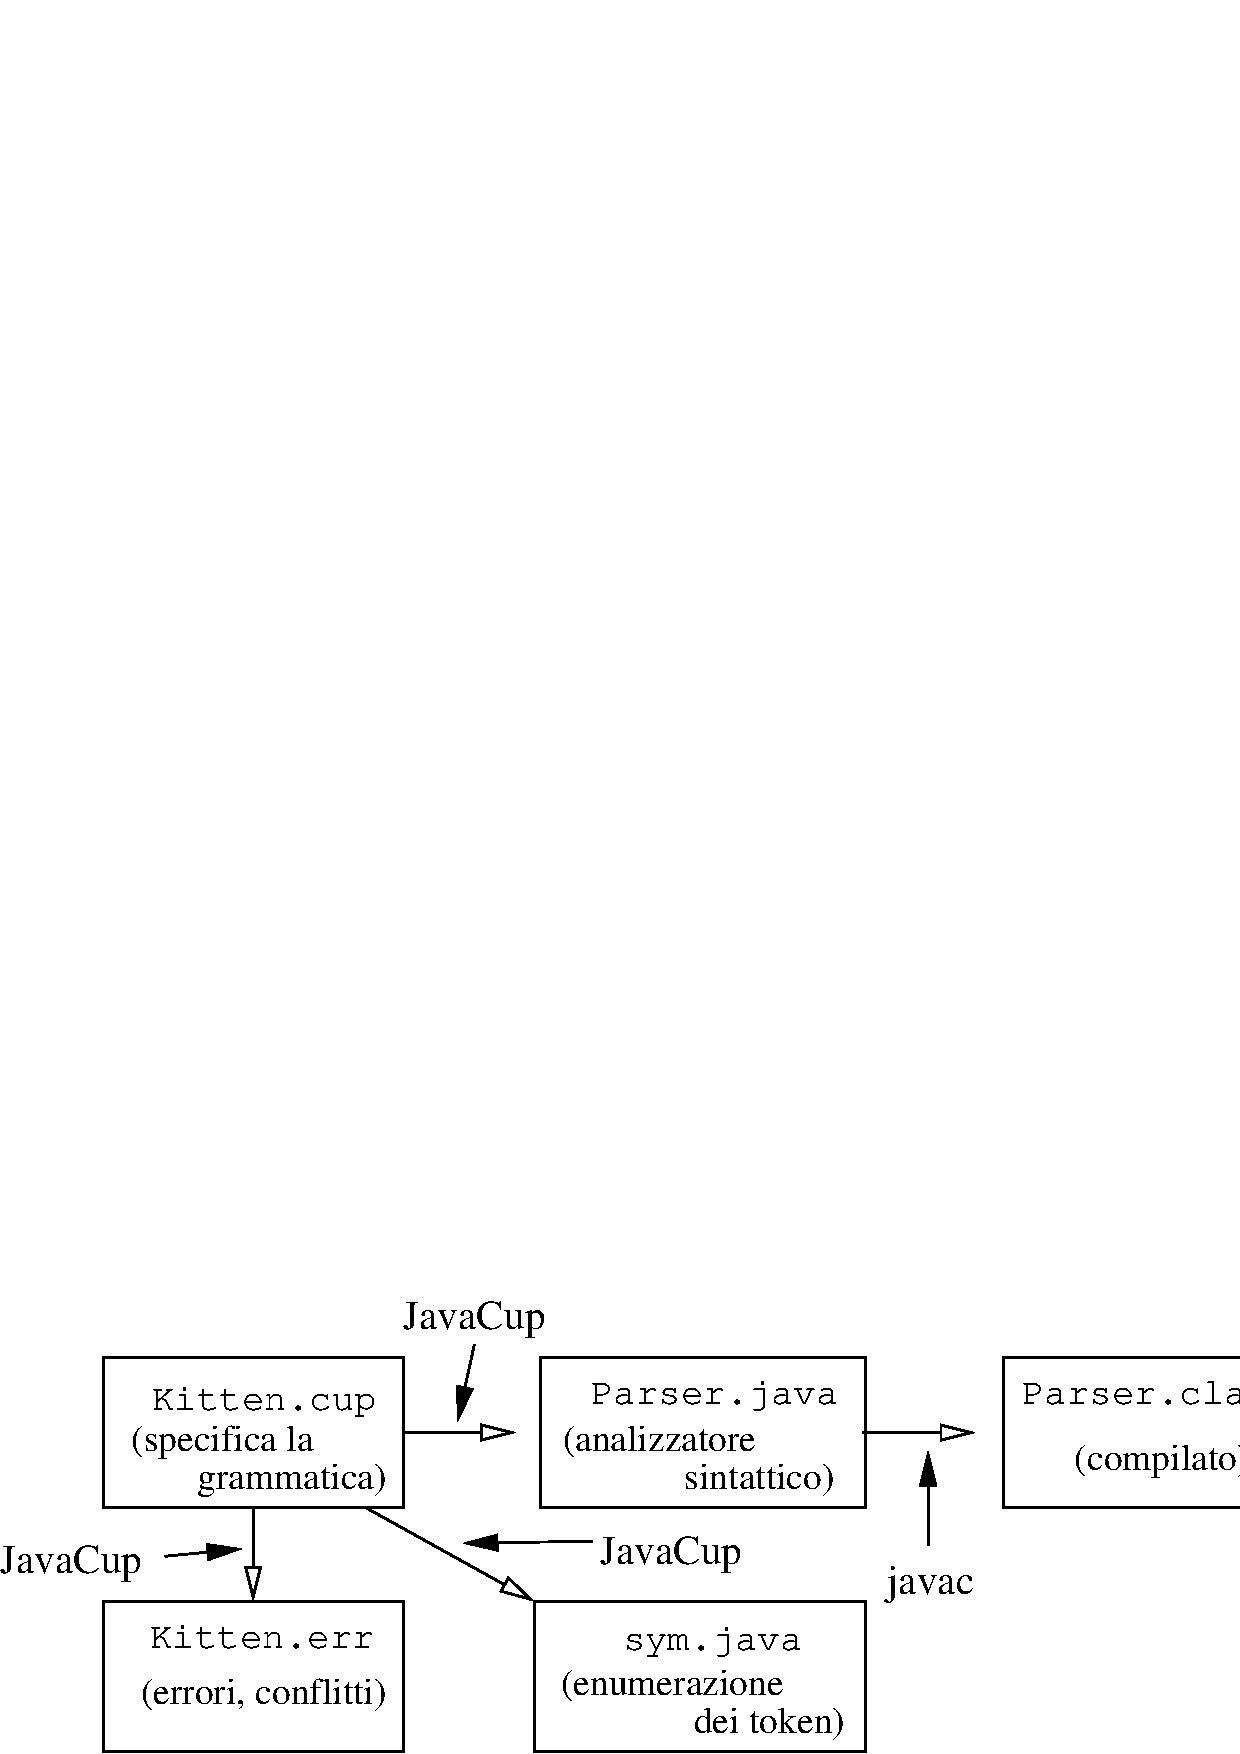
\includegraphics[scale=0.6]{pictures/java_cup.pdf}
\end{center}

\end{frame}

\begin{frame}[fragile]\frametitle{The grammar of Kitten for JavaCup: types}

\begin{verbatim}
  type ::=
     ID
   | BOOLEAN
   | INT
   | FLOAT
   | ARRAY OF type ;
\end{verbatim}

\begin{verbatim}
  typeplus ::=
     type
   | VOID ;
\end{verbatim}

\end{frame}

\begin{frame}[fragile]\frametitle{The grammar of Kitten for JavaCup: leftvalues and expressions}

\begin{verbatim}
  lvalue ::=
     ID                           // variable
   | exp DOT ID                   // a field of an object
   | exp LBRACK exp RBRACK ;      // an element of an array
\end{verbatim}

\begin{verbatim}
  exp ::=
     lvalue                       // a leftvalue
   | TRUE                         // literals...
   | FALSE  
   | INTEGER
   | FLOATING
   | STRING  
   | NIL     
   | NEW ID LPAREN expseq RPAREN  // object creation
   | NEW type LBRACK exp RBRACK   // array creation
\end{verbatim}

\end{frame}

\begin{frame}[fragile]\frametitle{The grammar of Kitten for JavaCup: more expressions}

\vspace*{-2ex}
\begin{verbatim}
   | exp AS type                     // cast into type
   | exp PLUS exp                    // arithmetic....
   | exp MINUS exp                   // AMBIGUITY
   | exp TIMES exp
   | exp DIVIDE exp
   | MINUS exp                       // unary minus
   | exp LT exp                      // comparisons...
   | exp LE exp                      // AMBIGUITY
   | exp GT exp
   | exp GE exp
   | exp EQ exp
   | exp NEQ exp
   | exp AND exp                     // logical operations...
   | exp OR exp                      // AMBIGUITY
   | NOT exp
   | exp DOT ID LPAREN expseq RPAREN // method call
   | LPAREN exp RPAREN ;             // parentheses
\end{verbatim}

\end{frame}

\begin{frame}[fragile]\frametitle{The grammar of Kitten for JavaCup: resolving the ambiguity}

Ambiguity can be resolved with a non-ambiguous grammar (complex, innatural) or with
\emph{precedence and associativity} rules:
%
\begin{verbatim}
  precedence left AND, OR;
  precedence left NOT;
  precedence nonassoc EQ, NEQ, LT, LE, GT, GE;
  precedence left PLUS, MINUS;
  precedence left TIMES, DIVIDE;
  precedence left UMINUS;
\end{verbatim}

\end{frame}

\begin{frame}[fragile]\frametitle{The grammar of Kitten for JavaCup: commands}

\begin{verbatim}
  command ::=
     lvalue ASSIGN exp  // assignment
   | type ID ASSIGN exp // variable declaration
   | RETURN             // return from void method
   | RETURN exp         // return from non-void method
   | IF LPAREN exp RPAREN THEN command  // conditionals...
   | IF LPAREN exp RPAREN THEN command ELSE command
   | WHILE LPAREN exp RPAREN command    // while loop
   | FOR LPAREN command SEMICOLON exp
       SEMICOLON command RPAREN command // for loop
   | LBRACE statements RBRACE          // local scope
   | exp DOT ID LPAREN expseq RPAREN;  // method call, again!
\end{verbatim}

\end{frame}

\begin{frame}[fragile]\frametitle{The grammar of Kitten for JavaCup: classes}

\begin{verbatim}
  class ::=
     CLASS ID LBRACE class_members RBRACE
   | CLASS ID EXTENDS ID LBRACE class_members RBRACE ;
\end{verbatim}

\begin{verbatim}
  class_members ::=
   | FIELD type ID class_members
   | CONSTRUCTOR LPAREN formals RPAREN command
       class_members
   | METHOD typeplus ID LPAREN formals RPAREN command
       class_members ;
\end{verbatim}

\end{frame}

\begin{frame}\frametitle{Building the abstract syntax}

Given a grammar and a program, JavaCup checks that the program agrees
with the grammar, otherwise it issues a syntax error. However, we want more:
we want to build the \emph{abstract syntax tree} of the program:

\begin{center}
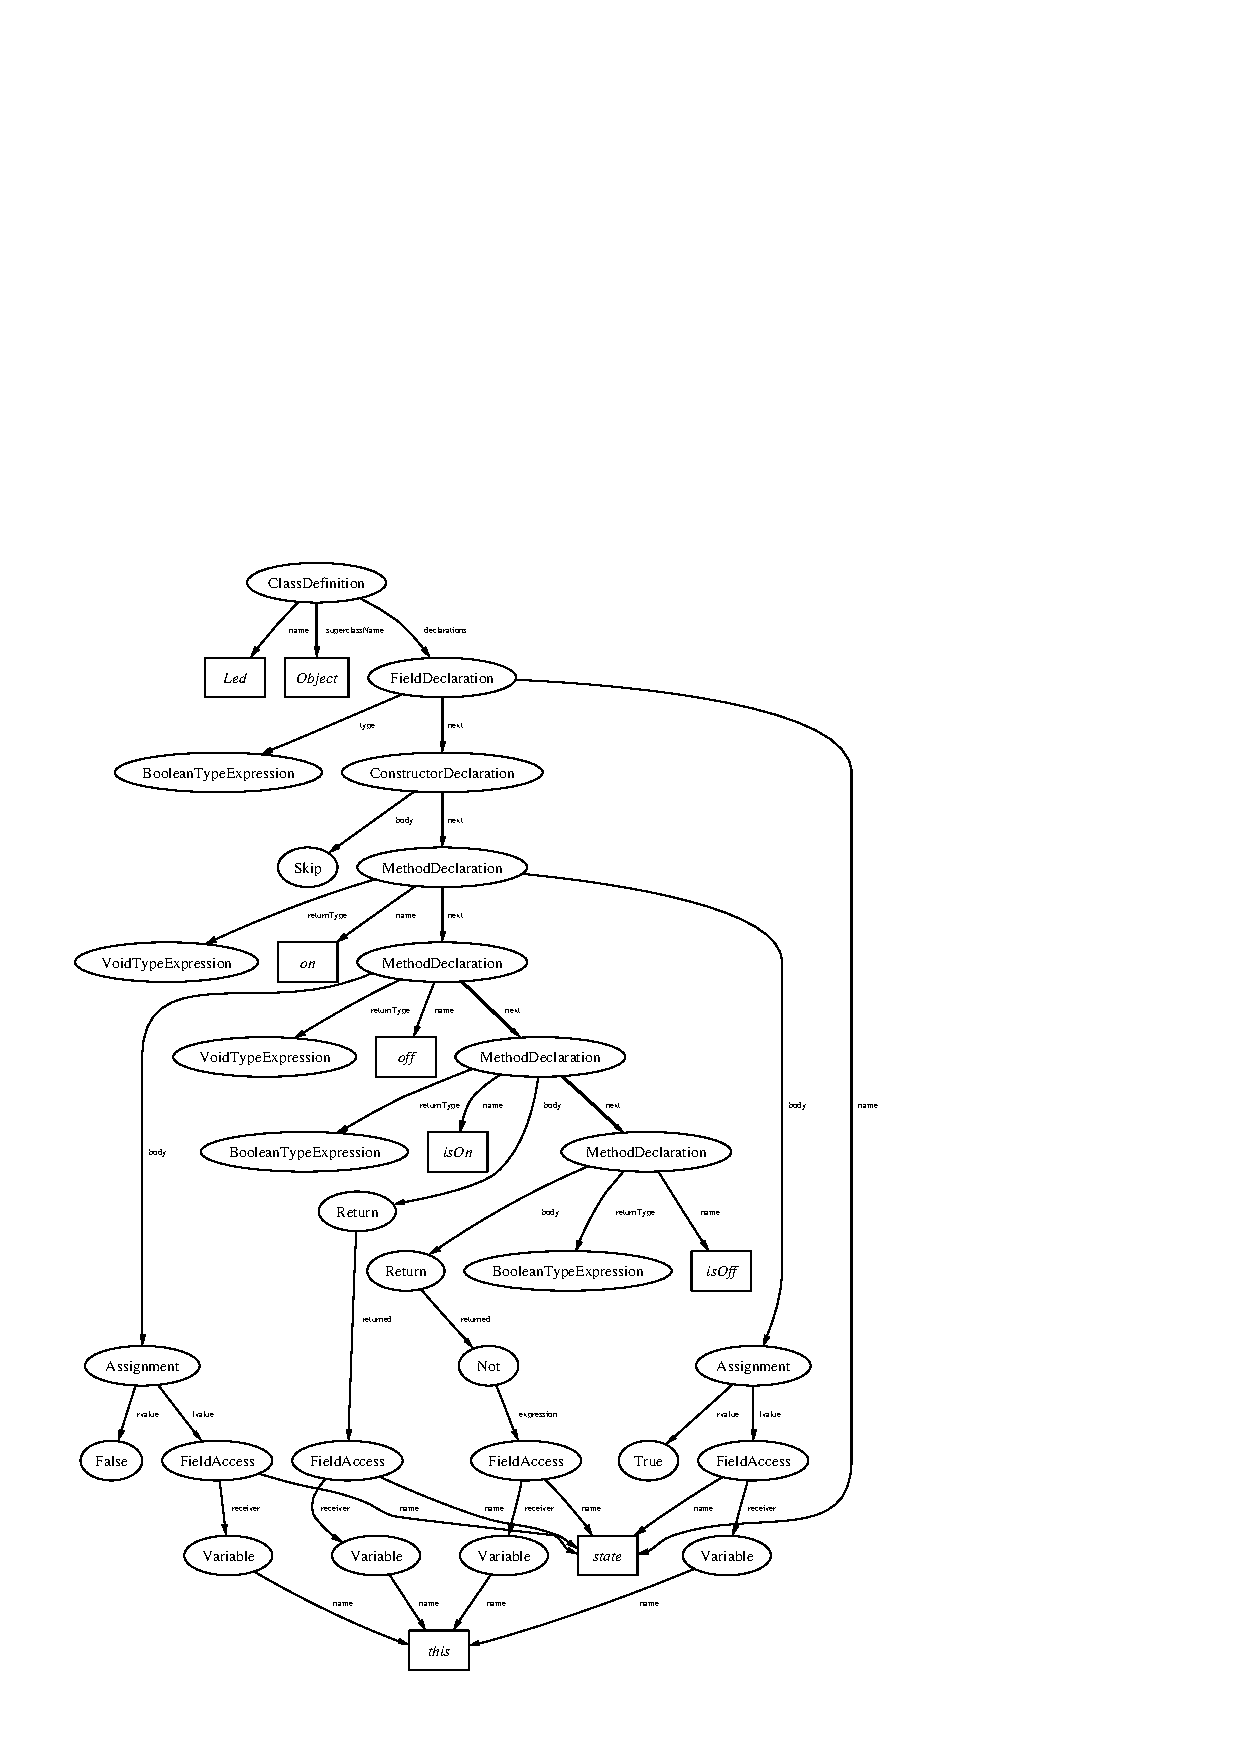
\includegraphics[scale=0.4]{pictures/led_logica.pdf}
\end{center}

\end{frame}

\begin{frame}[fragile]\frametitle{Semantical actions}

\begin{greenbox}{}
JavaCup allows one to specify \emph{semantical actions} that are fired when
a derivation is used in a parse tree. We will use this possibility to
build the syntax, recursively
\end{greenbox}

\end{frame}

\begin{frame}[fragile]\frametitle{Semantical actions for types}

\vspace*{-2ex}
\begin{verbatim}
type ::=
   ID
 | BOOLEAN
 | INT
 | FLOAT
 | ARRAY OF type ;
\end{verbatim}

become

\begin{verbatim}
type ::=
   ID:id     {: RESULT = new ClassTypeExpression(idleft, id); :}
 | BOOLEAN:b {: RESULT = new BooleanTypeExpression(bleft); :}
 | INT:i     {: RESULT = new IntTypeExpression(ileft); :}
 | FLOAT:f   {: RESULT = new FloatTypeExpression(fleft); :}
 | ARRAY:a OF type:t
   {: RESULT = new ArrayTypeExpression(aleft, t); :} ;
\end{verbatim}

\end{frame}

\begin{frame}[fragile]\frametitle{Classes for the abstract syntax: types}

\begin{greenbox}{}
The classes for the abstract syntax are organized into a hierarchy,
so that it will be simpler to share code among them in the future
\end{greenbox}

\begin{center}
\includegraphics[scale=0.53]{pictures/types_hierarchy.pdf}
\end{center}

\end{frame}

\begin{frame}[fragile]\frametitle{Classes for the abstract syntax: expressions}

\begin{center}
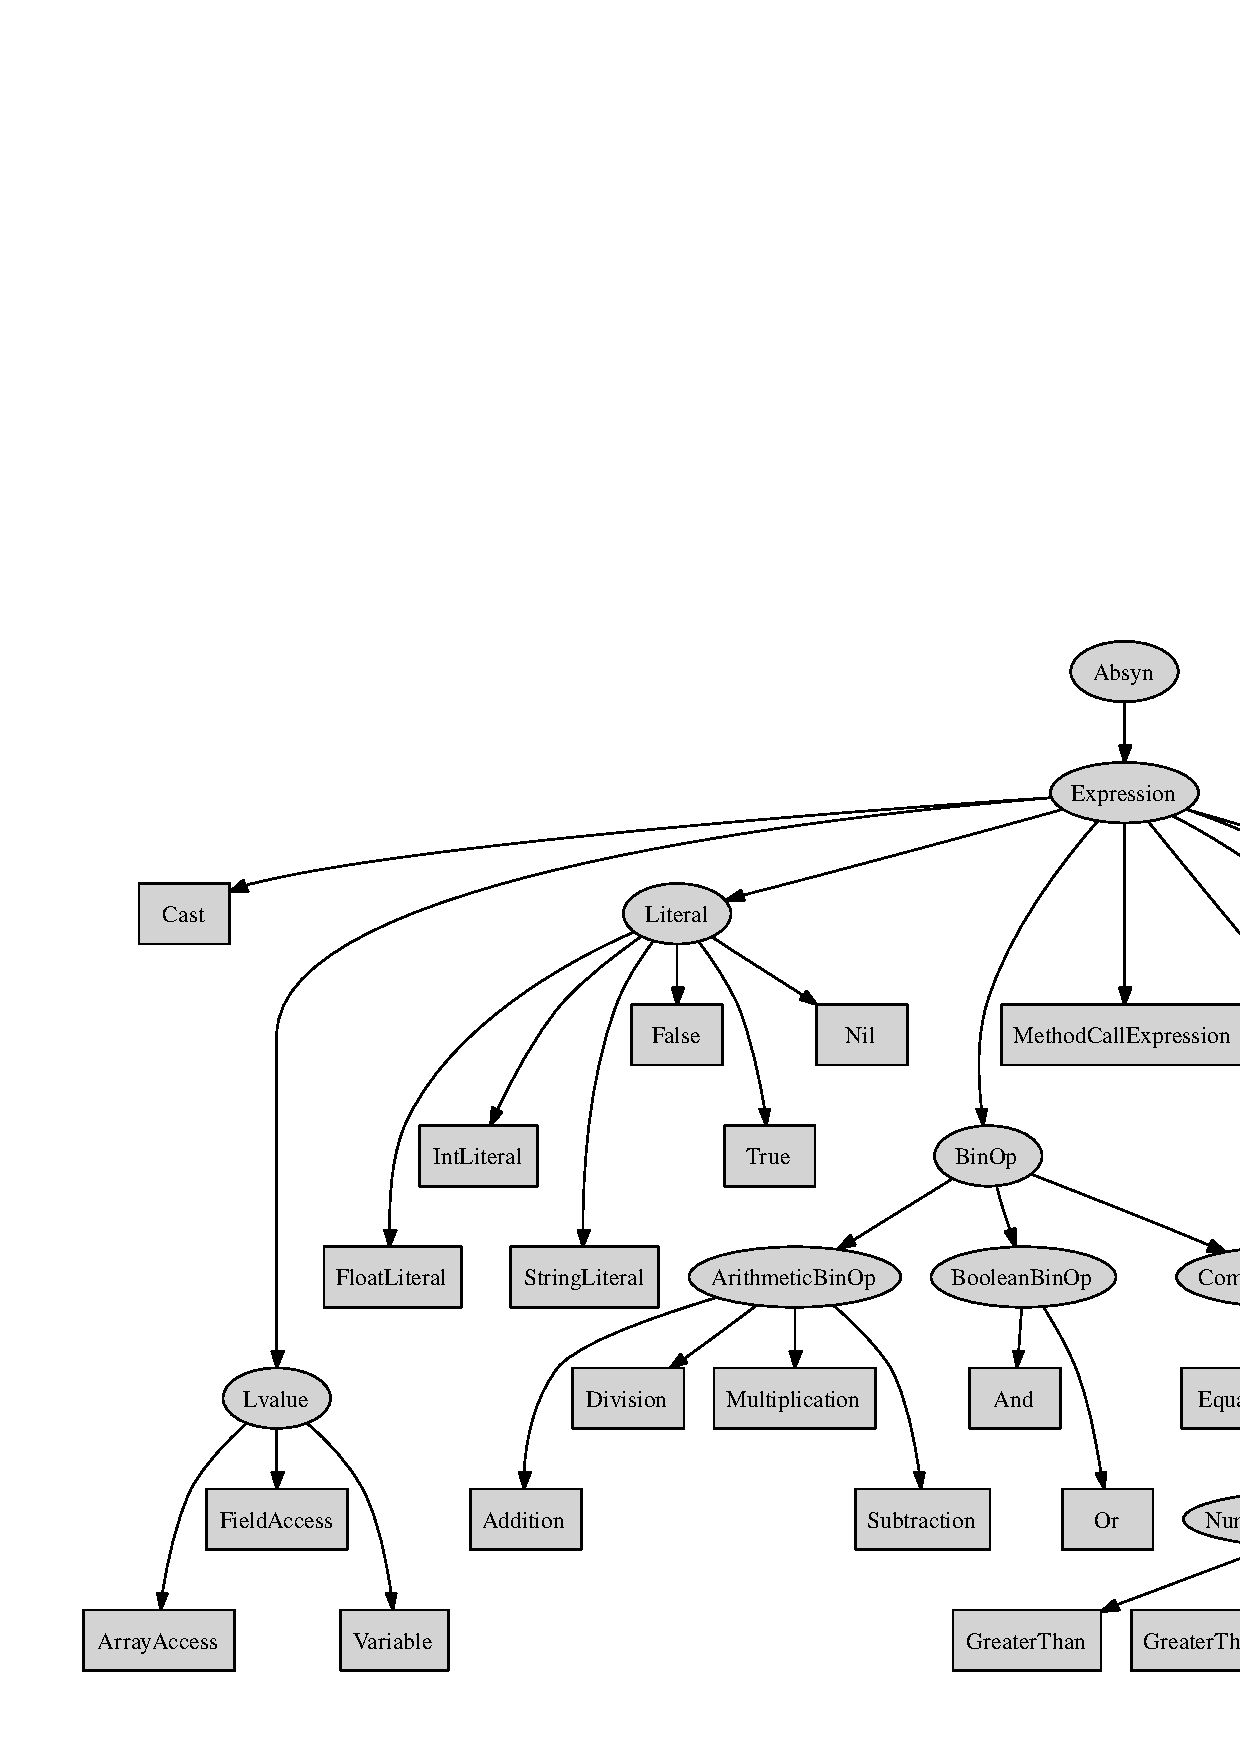
\includegraphics[scale=0.42]{pictures/expressions_hierarchy.pdf}
\end{center}

\end{frame}

\begin{frame}[fragile]\frametitle{Classes for the abstract syntax: commands}

\begin{center}
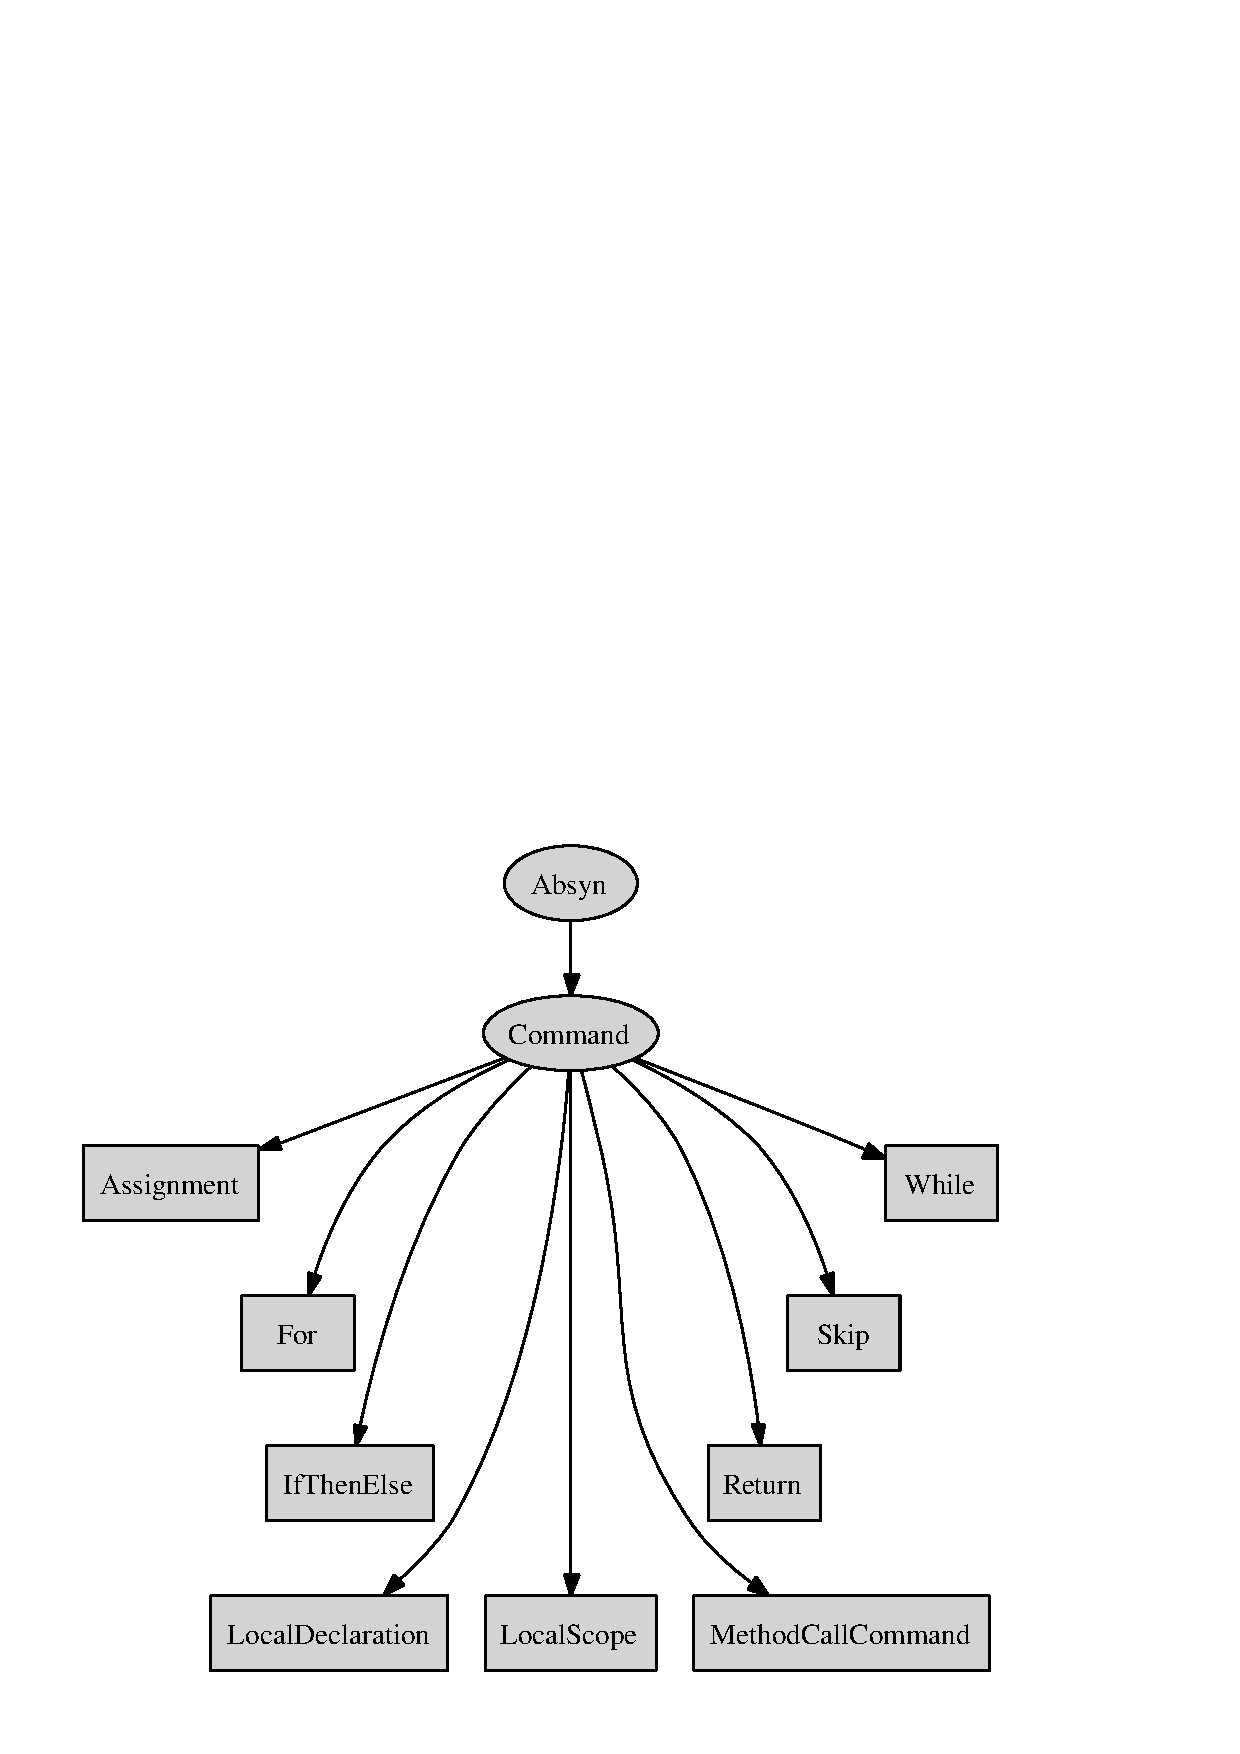
\includegraphics[scale=0.56]{pictures/commands_hierarchy.pdf}
\end{center}

\end{frame}

\begin{frame}
\frametitle{Semantical analysis}

\begin{center}
\begin{redbox}{Semantical analysis}
\begin{itemize}
\item \textbf{input:} abstract syntax tree
\item \textbf{output:} annotated abstract syntax tree
\item \textbf{error:} type error, unreachable code\ldots
\end{itemize}
\end{redbox}
\end{center}

\end{frame}

\begin{frame}\frametitle{Why do we need a semantical analysis phase?}

\begin{greenbox}{}
Grammars do not check for
%
\begin{itemize}
\item type consistency
\item undeclared variables
\item deadcode
\item using the return value of a void method
\item \ldots
\end{itemize}
%
\end{greenbox}

\mbox{}\\

The simplest implementation of those checks/inferences is through inductive
definitions, that automatically translate into Java code that
descends on the abstract syntax tree, recursively

\end{frame}

\newcommand{\cdc}{\vdash^{\mathsf{cdc}}}

\begin{frame}[fragile]\frametitle{Deadcode identification}

\begin{verbatim}
  while (x > 0) {
    x := x - 1;
    return;
    y := y + 1  <- a warning should be issued here
  }
\end{verbatim}

\[
  \boxed{command\cdc Boolean}
\]

$command\cdc true$ means that the execution of
$command$ definitely ends with the last command(s) of $command$.
\end{frame}

\begin{frame}\frametitle{Deadcode rules}

\[
  \frac{}{\mathtt{Return(x)}\cdc\mathit{true}}
\]

\mbox{}\\

\[
  \frac{}{\mathtt{Assignment(lvalue,rvalue)}\cdc\mathit{false}}
\]

\mbox{}\\

\[
  \frac{\mathtt{then}\cdc b_1\quad\mathtt{else}\cdc b_2}
    {\mathtt{IfThenElse(condition,then,else)}\cdc b_1\wedge b_2}
\]

\mbox{}\\

\[
  \frac{\text{if }\mathit{com}_1\cdc\mathit{true}\text{ issue a warning}
    \qquad\mathit{com}_2\cdc b}{\mathit{com}_1;\mathit{com}_2\cdc b}
\]

\mbox{}\\

\[
  \frac{\mathtt{body}\cdc b}
    {\mathtt{While(condition,body)}\cdc\mathit{false}}
\]

\end{frame}

\begin{frame}[fragile]\frametitle{Type inference and checking 1/4}

\[
  \boxed{\rho\vdash expression:type}
\]

\mbox{}\\

\[
  \frac{\rho(\mathit{name})\text{ is defined}}
    {\rho\vdash\mathtt{Variable(\mathit{name})}:\rho(\mathit{name})}
\]

\mbox{}\\

\[
  \frac{\begin{array}{c}
      \rho\vdash\mathit{receiver}:\kappa\quad\kappa\in\mathtt{ClassType}\\
      \mathit{field}=\kappa\mathtt{.fieldLookup(\mathit{name})}\quad
        \mathit{field}\not=\mathtt{null}
       \end{array}}
         {\rho\vdash\mathtt{FieldAccess(\mathit{receiver},\mathit{name})}:
          \mathit{field}\mathtt{.getType()}}
\]

\mbox{}\\

\[
  \frac{\rho\vdash\mathit{array}:t\quad t\in\mathtt{ArrayType}\quad
          \rho\vdash\mathit{index}:\mathtt{INT}}
         {\rho\vdash\mathtt{ArrayAccess(\mathit{array},\mathit{index})}:
          t\mathtt{.getElementsType()}}
\]

\end{frame}

\begin{frame}[fragile]\frametitle{Type inference and checking 2/4}

\[
 \frac{}
         {\rho\vdash\mathtt{False()}:\mathtt{BOOLEAN}}\qquad
 \frac{}
         {\rho\vdash\mathtt{True()}:\mathtt{BOOLEAN}}\qquad
 \frac{}
         {\rho\vdash\mathtt{Nil()}:\mathtt{NIL}}
\]

\[
  \frac{}
       {\rho\vdash\mathtt{IntLiteral()}:\mathtt{INT}}\qquad
  \frac{}
       {\rho\vdash\mathtt{FloatLiteral()}:\mathtt{FLOAT}}
\]

\[
  \frac{}
       {\rho\vdash\mathtt{StringLiteral(\mathit{value})}:
       \mathtt{ClassType.mk(STRING)}}
\]

 \[
    \frac{\rho\vdash\mathit{expression}:\mathtt{BOOLEAN}}
         {\rho\vdash\mathtt{Not(\mathit{expression})}:\mathtt{BOOLEAN}}
    \qquad
    \frac{\rho\vdash\mathit{expression}:t\quad t\le\mathtt{FLOAT}}
         {\rho\vdash\mathtt{Minus(\mathit{expression})}:t}
  \]

  \[
    \frac{
          \mathit{intoType}=\tau[\![\mathit{type}]\!]\quad
          \rho\vdash\mathit{expression}:\mathit{fromType}\quad
          \mathit{intoType} < \mathit{fromType}}
         {\rho\vdash\mathtt{Cast(\mathit{type},\mathit{expression})}:
          \mathit{intoType}}
  \]

\end{frame}

\begin{frame}[fragile]\frametitle{Type inference and checking 3/4}

\[
    \frac{\begin{array}{c}
          \mathtt{ClassType.mk(\mathit{className})}=\kappa\quad
            \rho\vdash\mathit{actuals}:\vec{\tau}\\
          \kappa\mathtt{.constructorsLookup(}\vec{\tau})=
            \{\mathit{constructor}\}
          \end{array}}
         {\rho\vdash\mathtt{NewObject(\mathit{className},\mathit{actuals})}:
          \kappa}
  \]
  \[
    \frac{\rho\vdash\mathit{elementsType}:t\quad\rho\vdash\mathit{size}:
          \mathtt{INT}}
         {\rho\vdash\mathtt{NewArray(\mathit{elementsType},\mathit{size})}:
          \mathtt{ArrayType.mk(\mathit{t})}}
  \]
  \[
     \frac{\begin{array}{c}
       \rho\vdash\mathit{receiver}:\kappa\quad\kappa\in\mathtt{ClassType}
         \quad\rho\vdash\mathit{actuals}:\vec{\tau}\\
       \kappa\mathtt{.methodsLookup(\mathit{name},}\vec{\tau})=
           \{\mathit{method}\}\quad
         r=\mathit{method}\mathtt{.getReturnType()}
           \quad r\not=\mathtt{VOID}
       \end{array}}
          {\rho\vdash\mathtt{MethodCallExpression(\mathit{receiver},
           \mathit{name},\mathit{actuals})}:r}
  \]

\[
    \frac{\rho\vdash\mathit{left}:t_l\quad
          \rho\vdash\mathit{right}:t_r\quad t_l\le\mathtt{FLOAT}
          \quad t_r\le\mathtt{FLOAT}}
         {\rho\vdash\mathtt{ArithmeticBinOp(\mathit{left},\mathit{right})}:
          t_l\mathtt{.leastCommonSupertype(\mathit{t_r})}}
  \]

  \[
    \frac{\rho\vdash\mathit{left}:t_l\quad
          \rho\vdash\mathit{right}:t_r\quad (\text{either }t_l\le t_r\text{ or }
          t_r\le t_l)}
         {\rho\vdash\mathtt{Equal(\mathit{left},\mathit{right})}:
           \mathtt{BOOLEAN}}
  \]

\end{frame}

\begin{frame}[fragile]\frametitle{Type inference and checking 4/4}

  \[
    \frac{t=\tau[\![\mathit{type}]\!]\quad\rho\vdash\mathit{initialiser}:i\quad 
          i\le t}
         {\rho\vdash\mathtt{LocalDeclaration(\mathit{type},\mathit{name},
          \mathit{initialiser})}:\rho[\mathit{name}\mapsto t]}
  \]

\[
    \frac{\rho\vdash\mathit{lvalue}:t_l\quad\rho\vdash\mathit{rvalue}:t_r
          \quad t_r\le t_l}
         {\rho\vdash\mathtt{Assignment(\mathit{lvalue},\mathit{rvalue})}:\rho}
  \]

 \[
    \frac{\rho\vdash\mathit{condition}:\mathtt{Type.BOOLEAN}\quad
          \rho\vdash\mathit{then}:\rho'\quad
          \rho\vdash\mathit{else}:\rho''}
         {\rho\vdash\mathtt{IfThenElse(\mathit{condition},\mathit{then},
          \mathit{else}):\rho}}
  \]
  \[
    \frac{\mathit{expression}\not=\mathtt{null}\quad
          \rho\vdash\mathit{expression}:t\quad
          \text{it is in a method that returns $r\ge t$}}
         {\rho\vdash\mathtt{Return(\mathit{expression})}:\rho}
  \]

  \[
    \frac{\rho\vdash\mathit{condition}:\mathtt{Type.BOOLEAN}\quad
          \rho\vdash\mathit{body}:\rho'}
         {\rho\vdash\mathtt{While(\mathit{condition},\mathit{body})}:\rho}
  \]

\end{frame}

\begin{frame}
\frametitle{Intermediate code generation}

\begin{center}
\begin{redbox}{Generation of the intermediate Kitten bytecode}
\begin{itemize}
\item \textbf{input:} annotated abstract syntax tree
\item \textbf{output:} Kitten bytecode
\end{itemize}
\end{redbox}
\end{center}

\mbox{}\\

\begin{pinkbox}{Why not Java bytecode instead?}
\begin{itemize}
\item JB is too low level
\item JB is only implicitly typed
\item JB uses integers for Booleans
\item JB has many optimized variants of the same instruction
\item \ldots
\end{itemize}
\end{pinkbox}

\end{frame}

\begin{frame}[fragile]
\frametitle{Intermediate code generation}

\begin{greenbox}{Intermediate Kitten bytecode}
\begin{verbatim}
  Led():                          isOn():
    return void                     load 0 of type Led
                                    getfield Led.state
  on():                             return boolean
    load 0 of type Led
    const true                    isOff():
    putfield Led.state              load 0 of type Led
    return void                     getfield Led.state
                                    neg boolean
  off():                            return boolean
    load 0 of type Led
    const false
    putfield Led.state
    return void
\end{verbatim}
\end{greenbox}

\end{frame}

\begin{frame}
\frametitle{Intermediate code generation}

\begin{greenbox}{Intermediate Kitten bytecode: loops}
\begin{center}
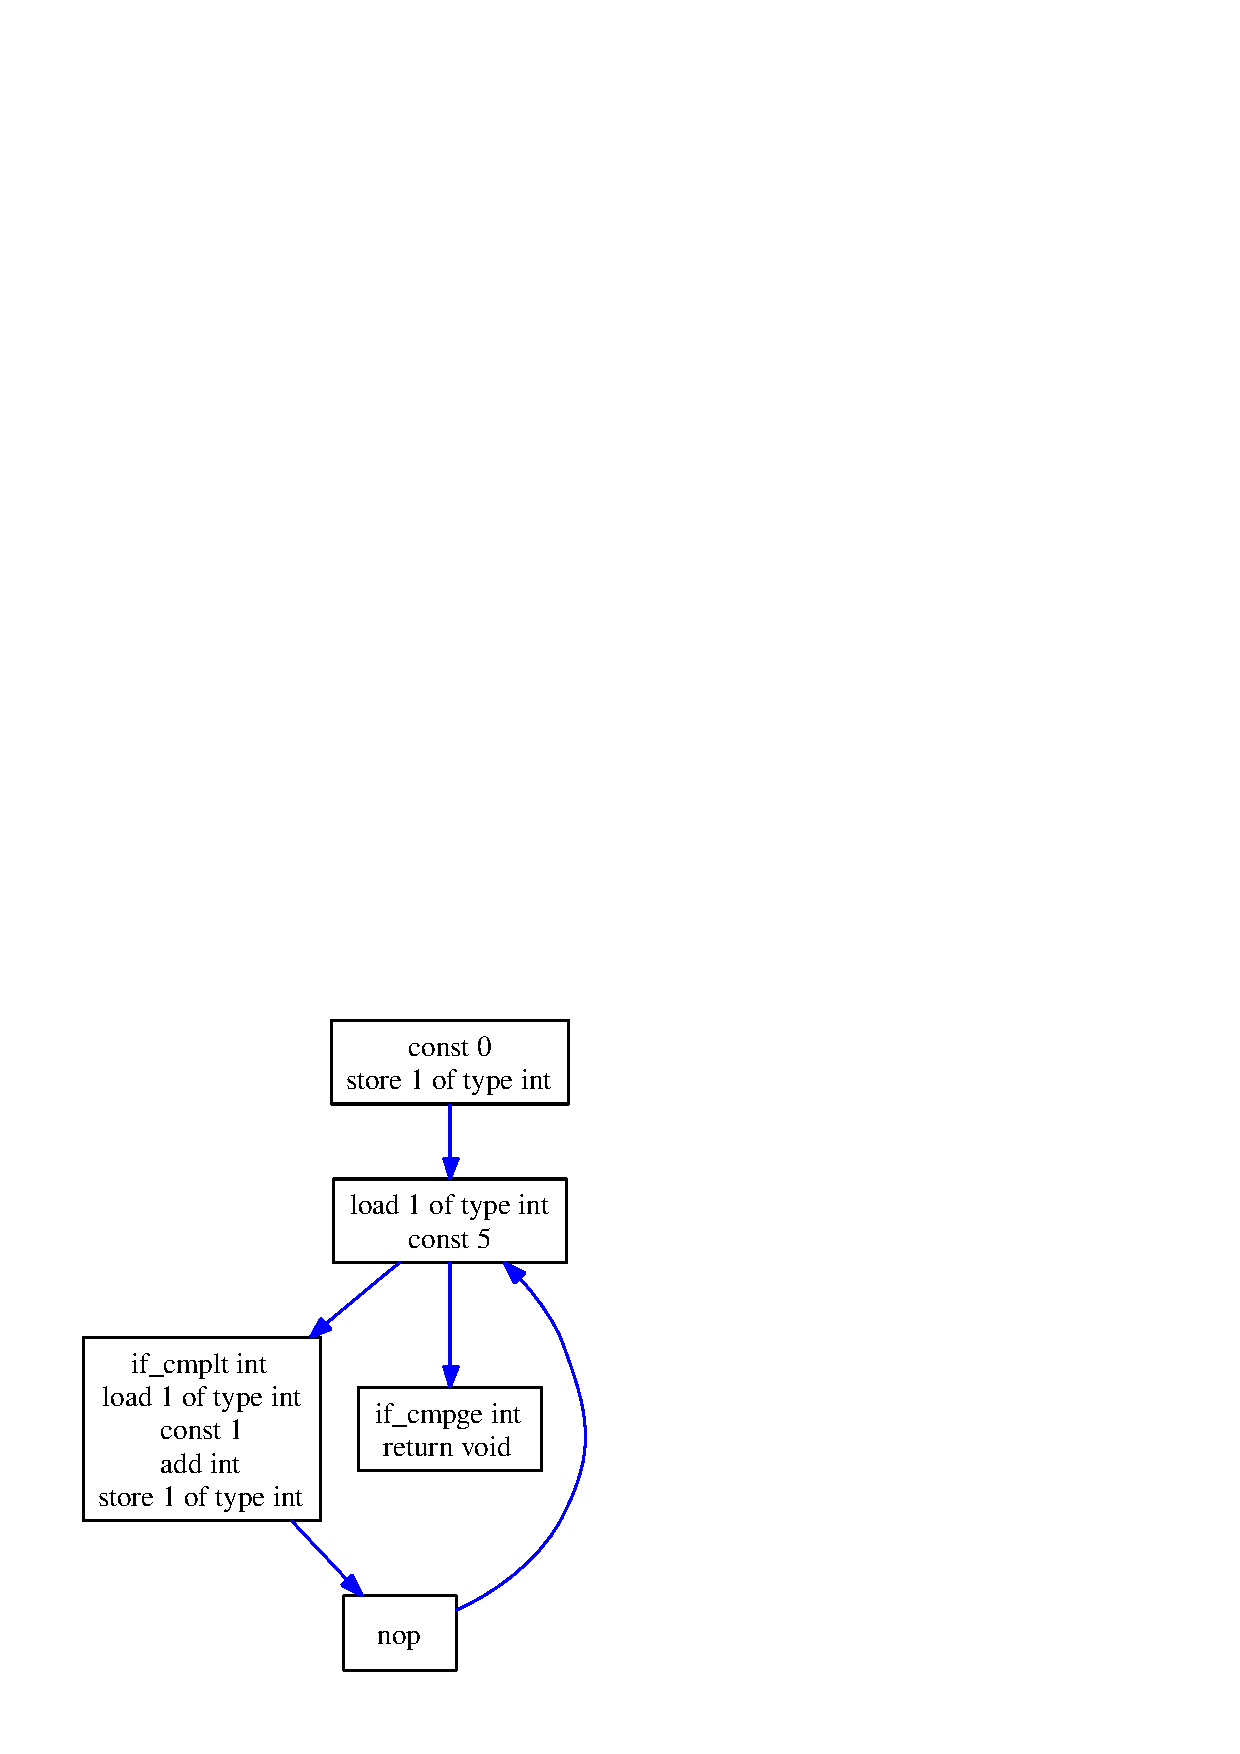
\includegraphics[scale=0.6]{pictures/loop.pdf}
\end{center}
\end{greenbox}
\end{frame}

\begin{frame}
\frametitle{Intermediate code generation for expressions 1/3}
\begin{enumerate}
\item leave the original stack untouched
\item push on top the value of the expression
\end{enumerate}

\mbox{}\\
For instance, the evaluation of $(e_1 \mathtt{\ and\ } e_2)$ looks like:
\begin{center}
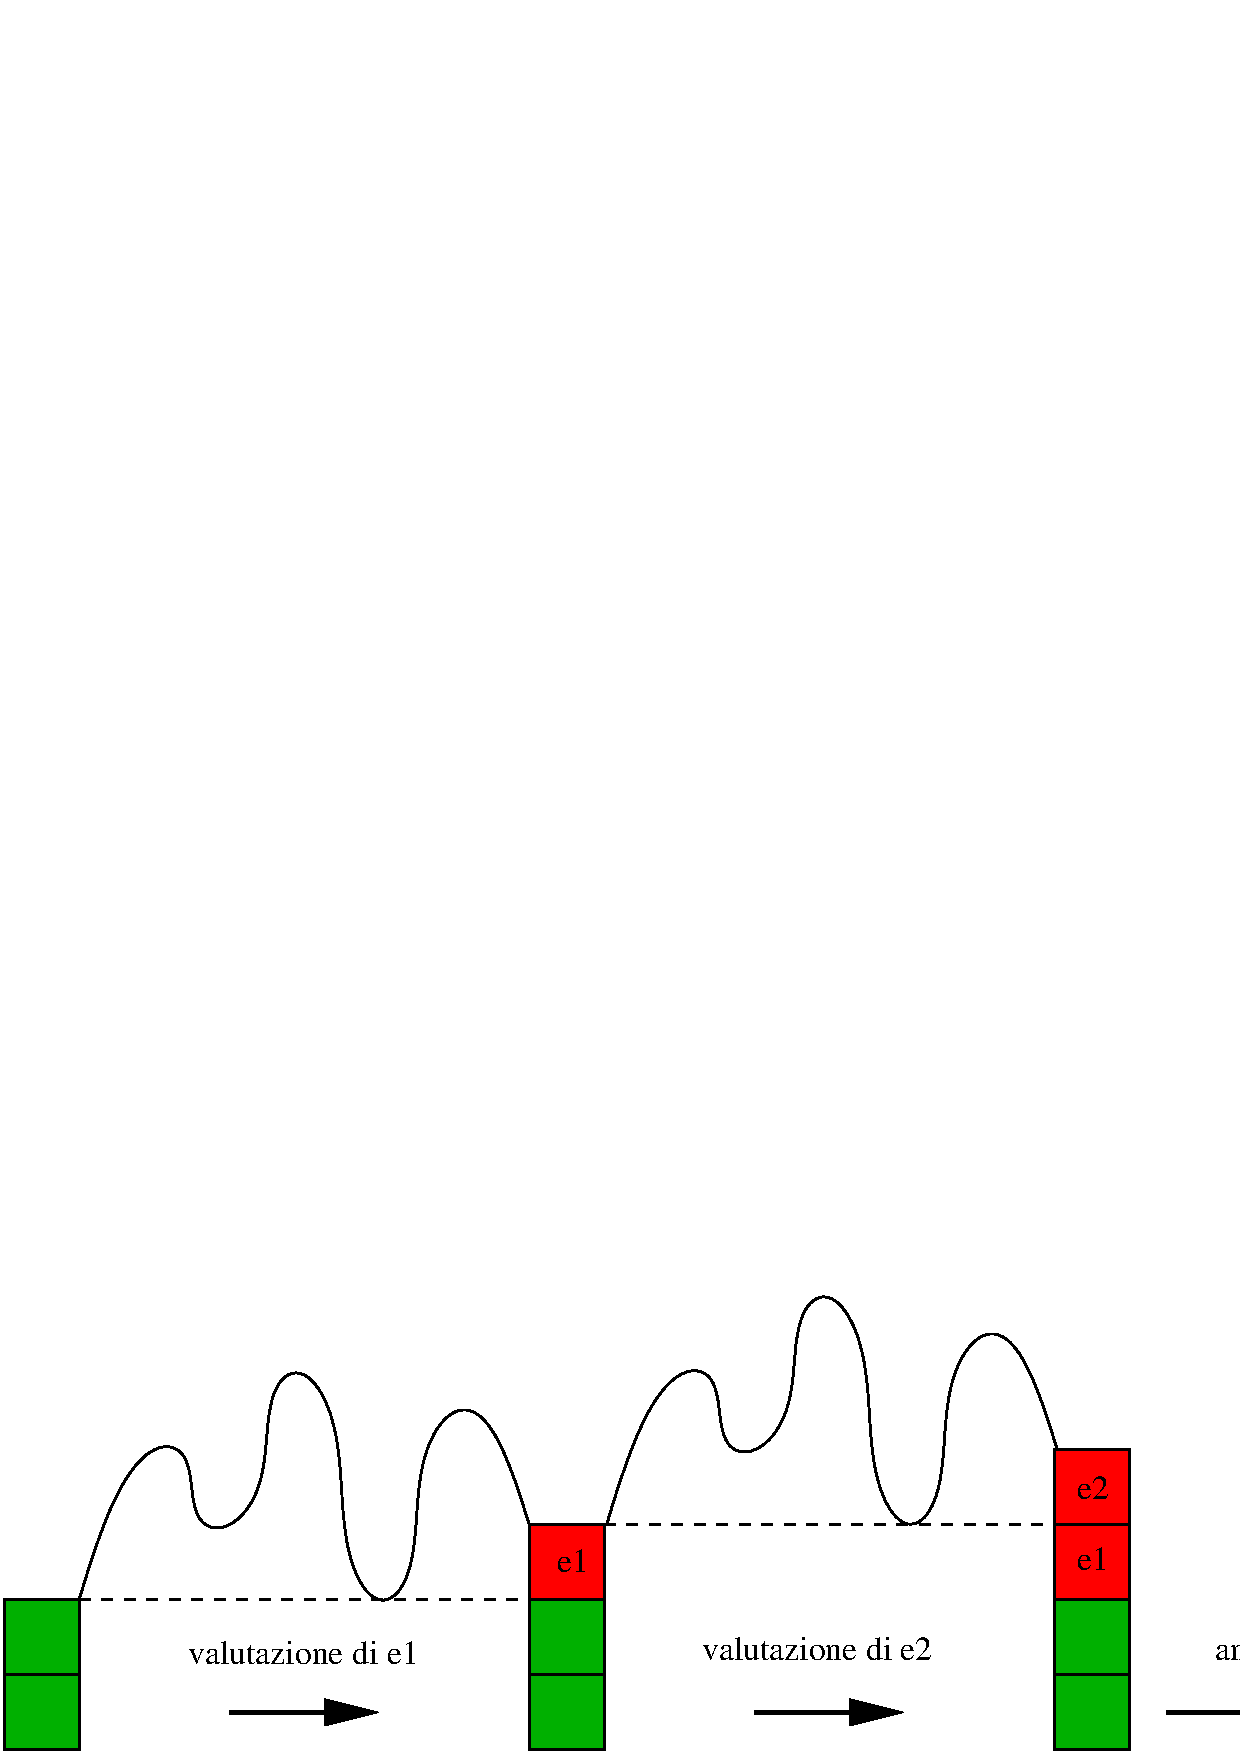
\includegraphics[scale=0.5]{pictures/importanza.pdf}
\end{center}

\end{frame}

\newcommand{\gen}[1]{\gamma[\![{#1}]\!]}
\newcommand{\gentwo}[2]{\gamma^{#1}[\![{#2}]\!]}

\begin{frame}
\frametitle{Intermediate code generation for expressions 2/3}

\[
  \boxed{\gen{\_}:\mathtt{expression}\mapsto
    \mathtt{block}\mapsto\mathtt{block}}
\]

\[
  \gen{\mathtt{True()}}(\beta)=\fbox{$\mathtt{const\ true}$}\to\beta
\]

\[
  \gen{\mathtt{Variable(\mathit{name})}}(\beta)=\fbox{\texttt{load $\mathit{num}$ of type $\tau$}}\to\beta
\]

\[
  \gen{\mathtt{And(\mathit{left},\mathit{right})}}(\beta)=
    \gen{\mathit{left}}\left(
      \gen{\mathit{right}}\left(\fbox{$\mathtt{and}$}\to\beta\right)\right)
\]

\[
  \gen{\mathtt{FieldAccess(\mathit{receiver},\mathit{name})}}(\beta)=
    \gen{\mathit{receiver}}\left(\fbox{\texttt{getfield $\mathit{field}$}}
    \to\beta\right)
\]

\begin{multline*}
   \gen{\mathtt{ArrayAccess(\mathit{array},\mathit{index})}}(\beta)\\
    =\gen{\mathit{array}}\left(\gen{\mathit{index}}\left(
    \fbox{$\mathtt{arrayload\ from\ array\ of\ }\tau$}\to\beta\right)\right)
\end{multline*}

\end{frame}

\begin{frame}
\frametitle{Intermediate code generation for expressions 3/3}

\[
  \gen{\mathtt{Cast(\mathit{\mathit{type},\mathit{expression}})}}(\beta)=
      \gen{\mathit{expression}}\left(\fbox{$\mathtt{cast\ from\ }\tau'\mathtt{\ into\ }\tau$}
        \to\beta\right)
\]

\[
  \gen{\mathtt{Addition(\mathit{left},\mathit{right})}}(\beta)=
    \gentwo{\tau}{\mathit{left}}\left(
      \gentwo{\tau}{\mathit{right}}\left(\fbox{$\mathtt{add}\ \tau$}
      \to\beta\right)\right)
\]

\begin{multline*}
  \gen{\mathtt{MethodCallExpression(\mathit{receiver},\mathit{name},
    \mathit{actuals})}}\\
  =\gen{\mathit{receiver}}\left(
    \gentwo{\vec{t}}{\mathit{actuals}}
    \left(\fbox{$\mathtt{virtualcall}\ \mathit{method}$}
    \to\beta\right)\right)
\end{multline*}

\begin{multline*}
  \gen{\mathtt{NewObject(\mathit{className},\mathit{actuals})}}(\beta)\\
    =\fbox{$\begin{array}{l}
      \mathtt{new}\ \kappa\\
      \mathtt{dup}\ \kappa
    \end{array}$}\to
   \gentwo{\vec{t}}{\mathit{actuals}}
   \left(\fbox{$\mathtt{constructorcall}\ \mathit{con}$}\to\beta\right)
\end{multline*}

\end{frame}

\begin{frame}
\frametitle{Intermediate code generation for Boolean expressions}

\[
  \gentwo{\mathit{test}}{\mathit{exp}}(\beta_{\mathit{true}})(\beta_\mathit{false})=
    \gen{\mathit{exp}}\left(
      \fbox{$\mathtt{nop}$}\,\,\langle
    \begin{array}{l}
        \fbox{$\mathtt{if\_true}$}\to\beta_{\mathit{true}}\\
        \fbox{$\mathtt{if\_false}$}\to\beta_\mathit{false}
    \end{array}
    \right)
\]

\end{frame}

\begin{frame}
\frametitle{Passive compilation of leftvalues}

\[
  \boxed{\gentwo{\mathit{passive}}{\mathit{lvalue},\mathit{rvalue}}(\beta)}
\]

\[
    \mathtt{Variable(\mathit{name})}
\]
\[
    \gentwo{\tau}{\mathit{rvalue}}\left(\fbox{$\mathtt{store}\ \mathit{num}\ \mathtt{of\ type\ }\tau$}\to\beta\right)
\]

\vspace*{2ex}
\[
    \mathtt{FieldAccess(\mathit{receiver},\mathit{name})}
\]
\[
    \gen{\mathit{receiver}}\left(
      \gentwo{\tau}{\mathit{rvalue}}\left(\fbox{$\mathtt{putfield}\ \mathit{field}$}\to\beta\right)\right)
\]

\vspace*{2ex}
\[
    \mathtt{ArrayAccess(\mathit{array},\mathit{index})}
\]
\[
    \gen{\mathit{array}}\left(\gen{\mathit{index}}\left(
      \gentwo{\tau}{\mathit{rvalue}}\left(\fbox{$\begin{array}{c}
      \mathtt{arraystore\ into}\\
      \mathtt{array\ of}\ \tau
      \end{array}$}\to\beta\right)\right)\right)
\]

\end{frame}

\begin{frame}
\frametitle{Intermediate code generation for the commands 1/2}

\begin{enumerate}
\item leave the original stack untouched
\end{enumerate}

\begin{center}
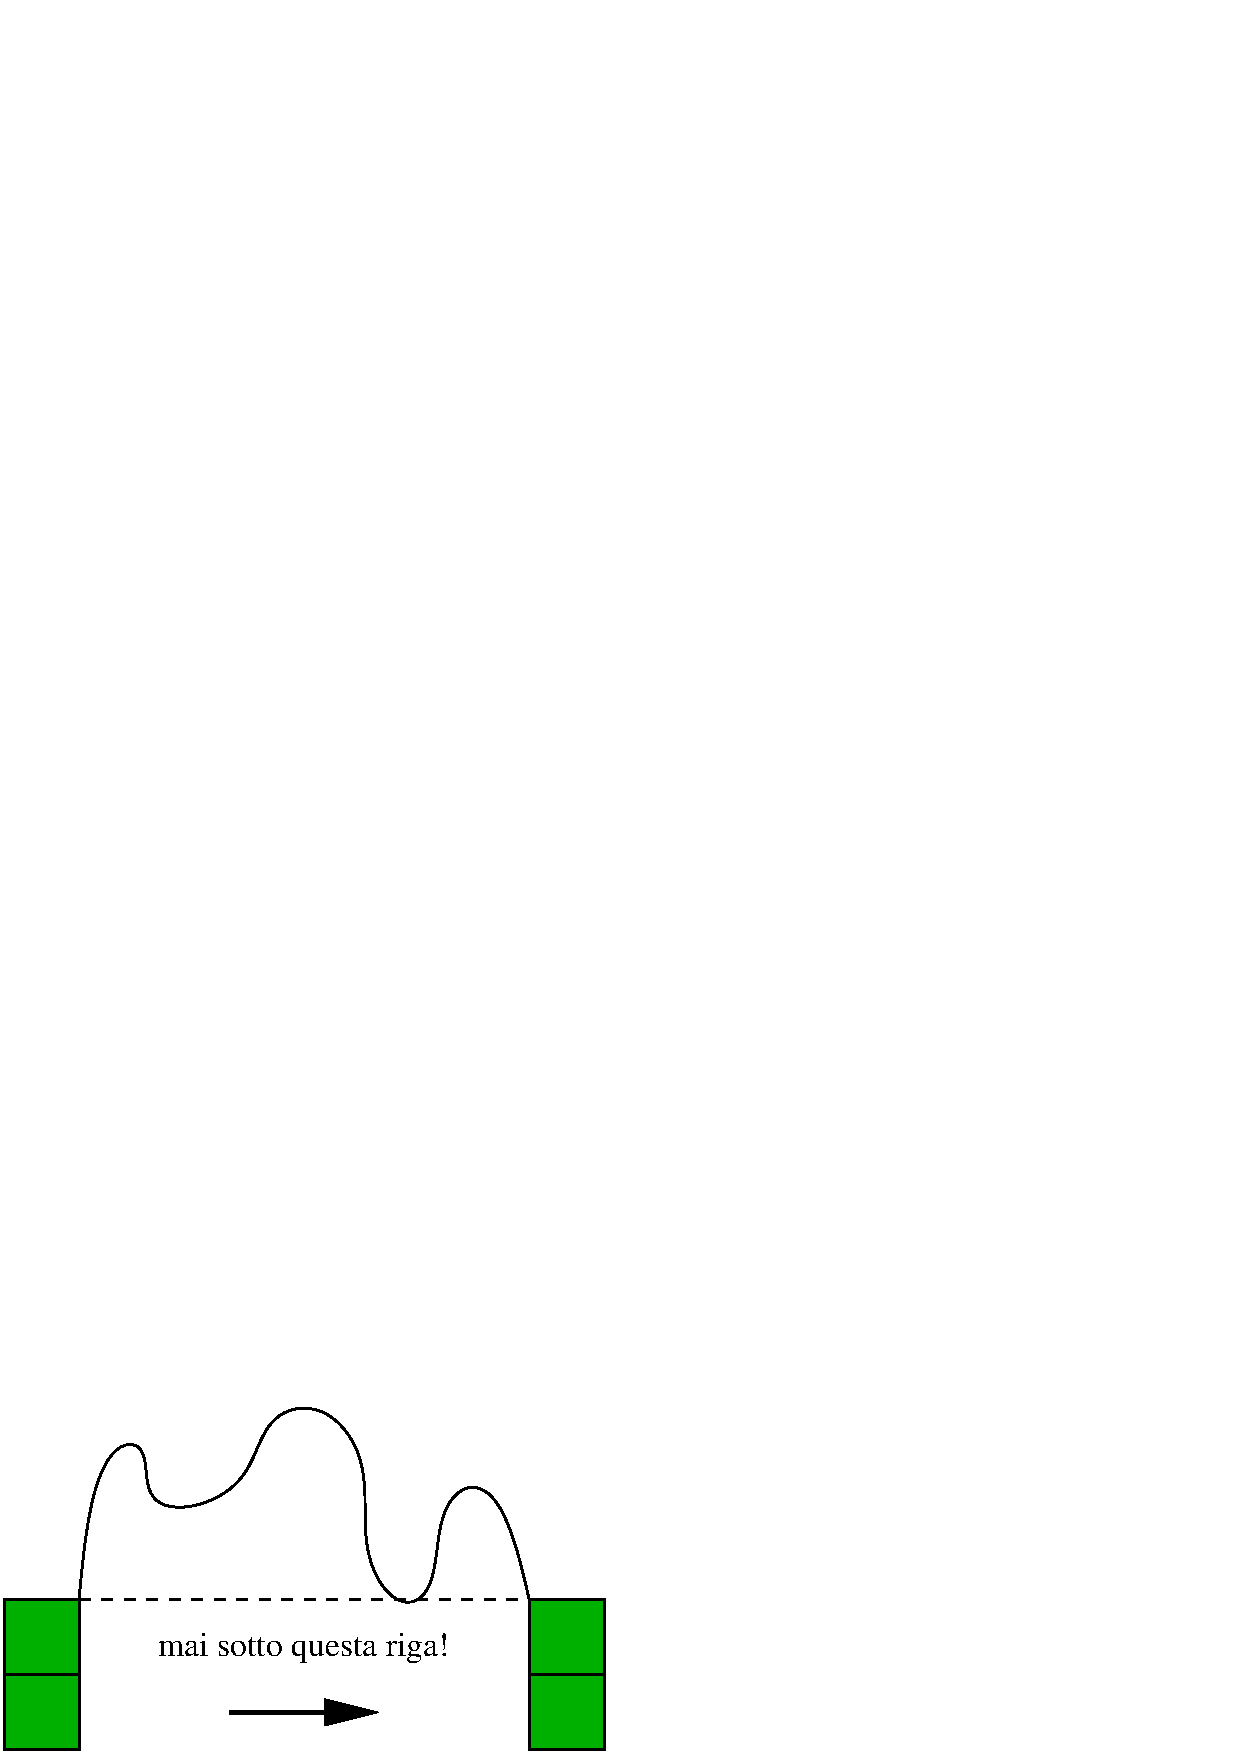
\includegraphics[scale=0.9]{pictures/russe2.pdf}
\end{center}

\end{frame}

\begin{frame}
\frametitle{Intermediate code generation for the commands 2/2}

\[
  \gen{\mathtt{Skip()}}(\beta)=\beta\qquad
    \gen{\mathtt{LocalScope(\mathit{body})}}(\beta)=
    \gen{\mathit{body}}(\beta)
\]

\[
   \gen{\mathtt{IfThenElse(\mathit{cond},\mathit{then},\mathit{else})}}
    (\beta)=\gentwo{\mathit{test}}{\mathit{cond}}
      (\gen{\mathit{then}}(\beta))(\gen{\mathit{else}}(\beta))
\]

\[
  \gen{\mathtt{Assignment(\mathit{lvalue},\mathit{rvalue})}}(\beta)=
    \gamma^\mathit{passive}\inter{\mathit{lvalue},\mathit{rvalue}}(\beta)
\]

\[
  \gen{\mathtt{While(\mathit{cond},\mathit{body})}}(\beta)=
    \underbrace{\fbox{$\mathtt{nop}$}}_\mathit{pivot}
    \to\gentwo{\mathit{test}}{\mathit{cond}}(\gen{\mathit{body}}(\mathit{pivot}))
    (\beta)
\]

\end{frame}

\begin{frame}
\frametitle{Java bytecode generation}

\begin{center}
\begin{redbox}{Generation of the object Java bytecode}
\begin{itemize}
\item \textbf{input:} Kitten bytecode
\item \textbf{output:} Java bytecode
\end{itemize}
\end{redbox}
\end{center}

\begin{pinkbox}{}
\begin{enumerate}
\item each Kitten bytecode is translated into one or more Java bytecodes,
      exploiting potential optimized variants
\item each block of Kitten bytecodes becomes a sequential snippet of Java bytecodes
\item such snippets are flattened into a linear sequence of Java bytecodes, by adding
      \texttt{goto}'s
\item everything is finally packaged into class files
\item a Java bytecode manipulation library such as BCEL does most of the work:
      \texttt{http://commons.apache.org/proper/commons-bcel}
\end{enumerate}
\end{pinkbox}

\end{frame}

\begin{frame}
\frametitle{Security guarantees of the Java bytecode}

\begin{greenbox}{A controlled low-level language}
\begin{itemize}
\item code cannot be modified at runtime $\Rightarrow$ \alert{no metamorphic code}
\item at each given program point,
      number and static types of stack elements and local variables are fixed
      and statically known,
      for all possible execution paths $\Rightarrow$
      \alert{strong types, you cannot blow up the stack}
\item casts are checked $\Rightarrow$ \alert{you cannot pretend that a frog is a prince}
\item unitialized local variables cannot be used $\Rightarrow$
      \alert{you cannot exploit stale values}
\item new objects cannot be used before calling one of their constructors
      $\Rightarrow$ \alert{you cannot forge raw data}
\item all jumps go to static targets, inside the same method
      $\Rightarrow$ \alert{you cannot dynamically build your jump targets}
\end{itemize}
\end{greenbox}

\begin{center}
Identical constraints hold for the Dalvik Android bytecode
\end{center}

\end{frame}

\end{document}
